\subsection{Справочник <<Технологические карты>>}
\label{spr:Design}


\subsubsection{Описание предметной области}

Справочник <<Технологические карты>> содержит информацию о технологических картах на изготовление готовой продукции. Список полей элемента справочника соответствует набору параметров технологической карты и включает в себя все необходимые данные о требованиях к изготовлению изделия. 
	
Справочник уже существует в СИСТЕМЕ, требуется внести изменения в его работу.

 \subsubsection{Атрибуты}

% Добавить новые атрибуты.
% \pc
% \begin{longtable}{|p{4cm}|p{4cm}|p{8cm}|}
% \hline
% {\bf Наименование} & {\bf Тип данных} &  {\bf Комментарий} \endhead
%     \hline
%     Группа сложности & Справочник. Группы сложности  & Группа сложности изделия. Необходима для отчета ''Показатели работы''\\
%     \hline
%   \caption{Новые поля Справочника <<Технологические карты>>}
%  \label{tab:Design}
% \end{longtable}
% %
Изменить атрибуты атрибуты.
\pc
\begin{longtable}{|p{4cm}|p{4cm}|p{8cm}|}
\hline
{\bf Наименование} & {\bf Тип данных} &  {\bf Комментарий} \endhead
    \hline
    ДлинаИзделия & Тип число (10,1)  & Добавить дробную часть\\
    \hline
    ШиринаИзделия & Тип число (10,1)  & Добавить дробную часть\\
    \hline
    ВысотаИзделия & Тип число (10,1)  & Добавить дробную часть\\
    \hline
    ПлощадьРазвертки & Тип число (13,3)  & Добавить дробную часть\\
    \hline
    ВысотыСтопыНаГА & Тип число (10,0)  & Высота стопы на ГА\\
    \hline    
    Дно & Флаг  & Признак необходимости добавления на дно прокладочных листов.\\
    \hline
    Процент выпуска  & Тип число (10,0)  & Параметр указывает процент от задания, при выполнении которого его можно считать выполненным \\
    \hline    
  \caption{Справочника <<Технологические карты>>}
 \label{tab:Design2}
\end{longtable}
%


% На форме необходимо добавить следующие поля.

% \pc
% \begin{longtable}{|p{8cm}|p{3cm}|p{5cm}|}
% \hline
% {\bf Наименование} & {\bf Тип данных} &  {\bf Комментарий} \endhead
%     % \hline
%     % (???) Вес нетто (ВесНетто) & Булево &  Вкладка <<Бирка>> \\
%     % \hline
%     % (???) Вес брутто (ВесБрутто) & Булево &  Вкладка <<Бирка>> \\
%     \hline
%     Вес Нетто & Числовое поле, кратность - целое число & Вкладка <<Бирка>> \\
%     \hline
%     Вес Брутто & Числовое поле, кратность - целое число & Вкладка <<Бирка>> \\
%     \hline
   
%    \caption{Новые поля на форме <<Технологическая карта>>}
%   \label{tab:Specification}
% \end{longtable}
% %\clearpage



% В справочнике должны быть добавлены следующие поля.

\subsubsection{Функциональные требования}

\point{Форма редактирования}

Добавить новые параметры в форму редактирования.

 
%  ПРОРАБОТАТЬ РАЗРАБОТКУ НОВОГО КОДА ТК!

\bigskip


\subpoint{Учет высоты стопы}

Добавить параметр ВысотыСтопыНаГА для передачи параметра на гофроагрегат.
В случае заполненного значения в технологической карте при выгрузке данных в гофроагрегат должно быть взято значение из технологической карты.
В противном случае значение определяется по профилю гофры из справочника ''Профили''. 

% В справочнике вариантов исполнения на странице с параметрами оставить параметры ''Припуск по длине'', ''Припуск по ширине'', разрешать пользователю указывать значения параметров, но изменить процедуру автоматического расчета развертки изделия в техкарте: перестать выводить эти параметры на схеме и не прибавлять из значения к получившемуся размеру развертки.

% Модифицировать правило создания заготовки в технологической карте.
% При создании заготовки в качестве длины заготовки необходимо брать длину развертки изделия и прибавлять к ней (если указано) величину припуска из варианта исполнения, к ширине заготовки прибавлять величину припуска по ширине.

% \bigskip

\point{Печатная форма ''Технологической карты''. Полная}


 Изменить печатную форму полной технологической карты, которая должна формироваться из формы редактирования справочника.
 Внешний вид допустимо оставить близким к тому, какой используется в СИСТЕМЕ, но обеспечить вывод всех полей, представленных на примере техкарты, используемой на ПРЕДПРИЯТИИ, согласно рис. \ref{pic:Tk_1} - \ref{pic:Tk_4}.
%   (добавлено новое поле ''Содержвание штампа'').

 
% Список корректировок.
% \begin{itemize}
%     \item На первой странице заголовок таблицы с пантонами заменить на ''Цвет, наименования'';
%     \item На третьей странице добавить вывод полей ''Лент по длине'' и ''Лент по ширине'';
%     \item На четвертой странице (страница заготовки). Переименовать поле ''Изделий на штампе'' в  ''Изделий в заготовке''. Добавить вывод полей ''Площадь заготовки, м2'' и ''Площадь заготовки на одно изделие, м2'' (вычисляется как площадь заготовки, деленная на количество изделий в заготовке)
% \end{itemize}


% Поле ''Площадь заготовки'' должна рассчитываться по размерам заготовки (длина с припуском, ширина с припуском).


\begin{figure}
  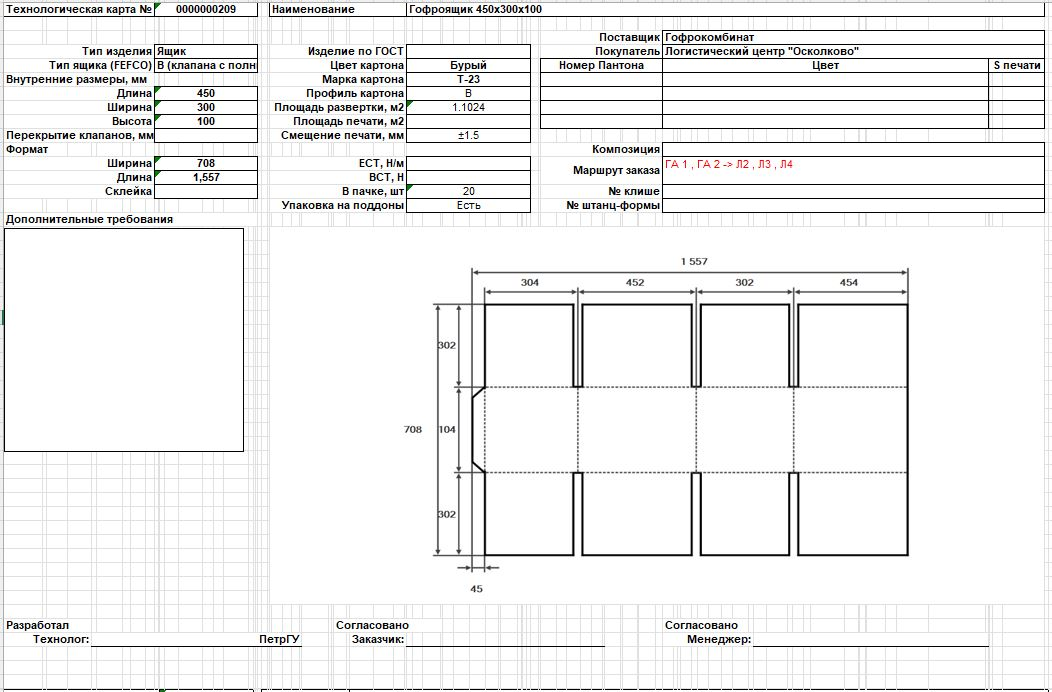
\includegraphics[height=0.8\textheight, width=\textwidth, angle=90,
  keepaspectratio] {50_Pics/Tk_1.JPG}
  \caption{Печатная форма Технологическая карта}
  \label{pic:Tk_1}
\end{figure}

\begin{figure}
\begin{center}
  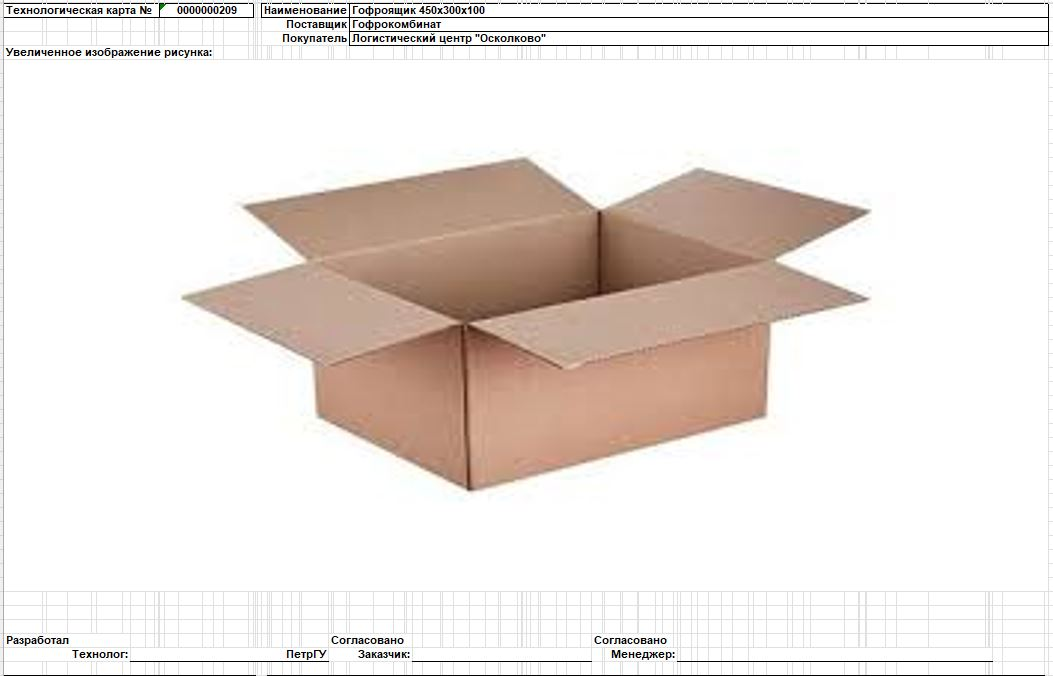
\includegraphics[height=0.7\textheight, width=\textwidth, angle=90,
  keepaspectratio]{50_Pics/Tk_2.JPG}
\end{center}
  \caption{Печатная форма Технологическая карта. Страница 2}
  \label{pic:Tk_2}
\end{figure}

\begin{figure}
\begin{center}
  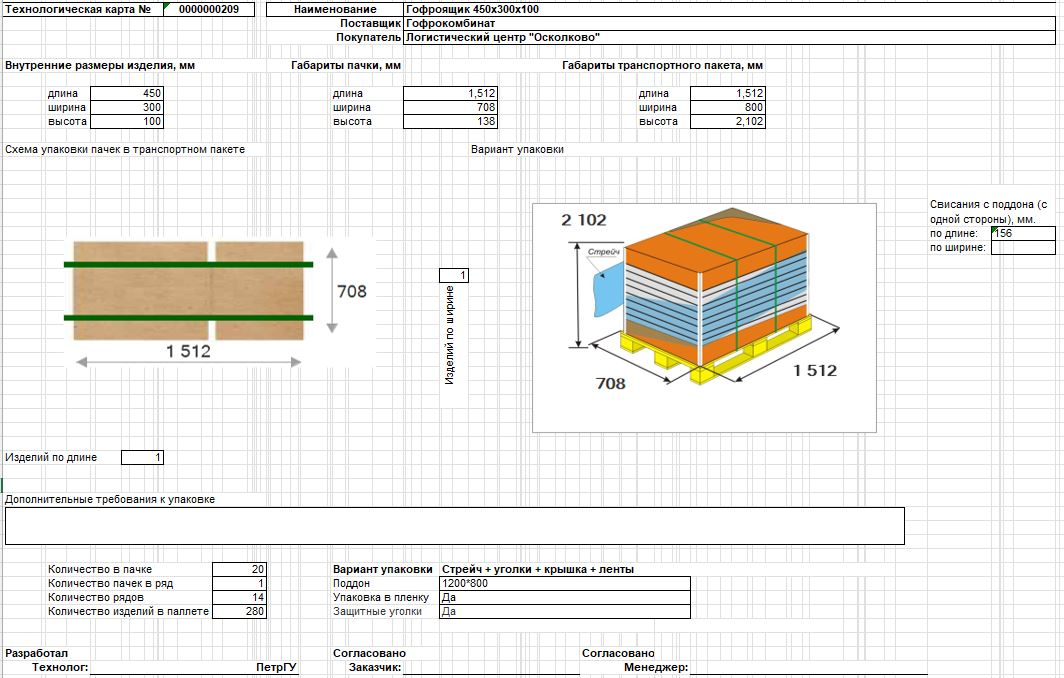
\includegraphics[height=0.7\textheight, width=\textwidth, angle=90,
  keepaspectratio]{50_Pics/Tk_3.JPG}
\end{center}
  \caption{Печатная форма Технологическая карта. Страница 3}
  \label{pic:Tk_3}
\end{figure}

\begin{figure}
\begin{center}
  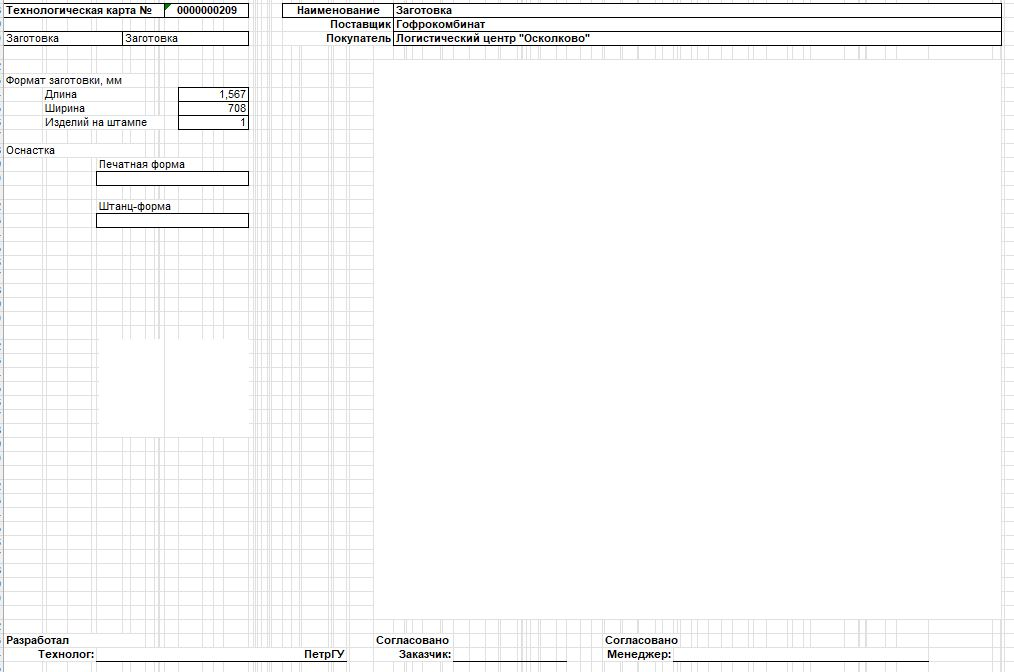
\includegraphics[height=0.7\textheight, width=\textwidth, angle=90,
  keepaspectratio]{50_Pics/Tk_4.JPG}
\end{center}
  \caption{Печатная форма Технологическая карта. Страница 4}
  \label{pic:Tk_4}
\end{figure}
\clearpage


\point{Форма ''Технологическая карта''. Вариант упаковки}

При выборе варианта упаковки заполнять реквизит ''Дно''.

% Форма уже существует в СИСТЕМЕ, требуется внести изменения в ее работу.



% \subsubsection{Функциональные требования}

% \point{Форма редактирования}

% (Точно нужно так перегружать???) Правило: Если ВесНетто = активен, доступно для редактирования поле <<Вес нетто>>, данные параметра <<Вес нетто>> выводить на бирку (Поле ВесНетто).
% Если ВесБрутто = активен, доступно для редактирования поле <<Вес брутто>>, данные параметра <<Вес брутто>> выводить на бирку (поле ВесБрутто).
% Если ВесНетто, ВесБрутто = неактивен, на бирке скрывать наименование полей ВесНетто и ВесБрутто. Пример бирки на готовую продукцию с отсутствием информации о весе нетто и брутто представлен на рис. \ref{pic:БиркаГП2}.

